
\newgeometry{top=3.5in,bottom=4in,right=1.0in,left=1.0in}
\begin{titlepage} 

    \tikz[overlay, remember picture] \node[opacity=0.8] at (current page.center){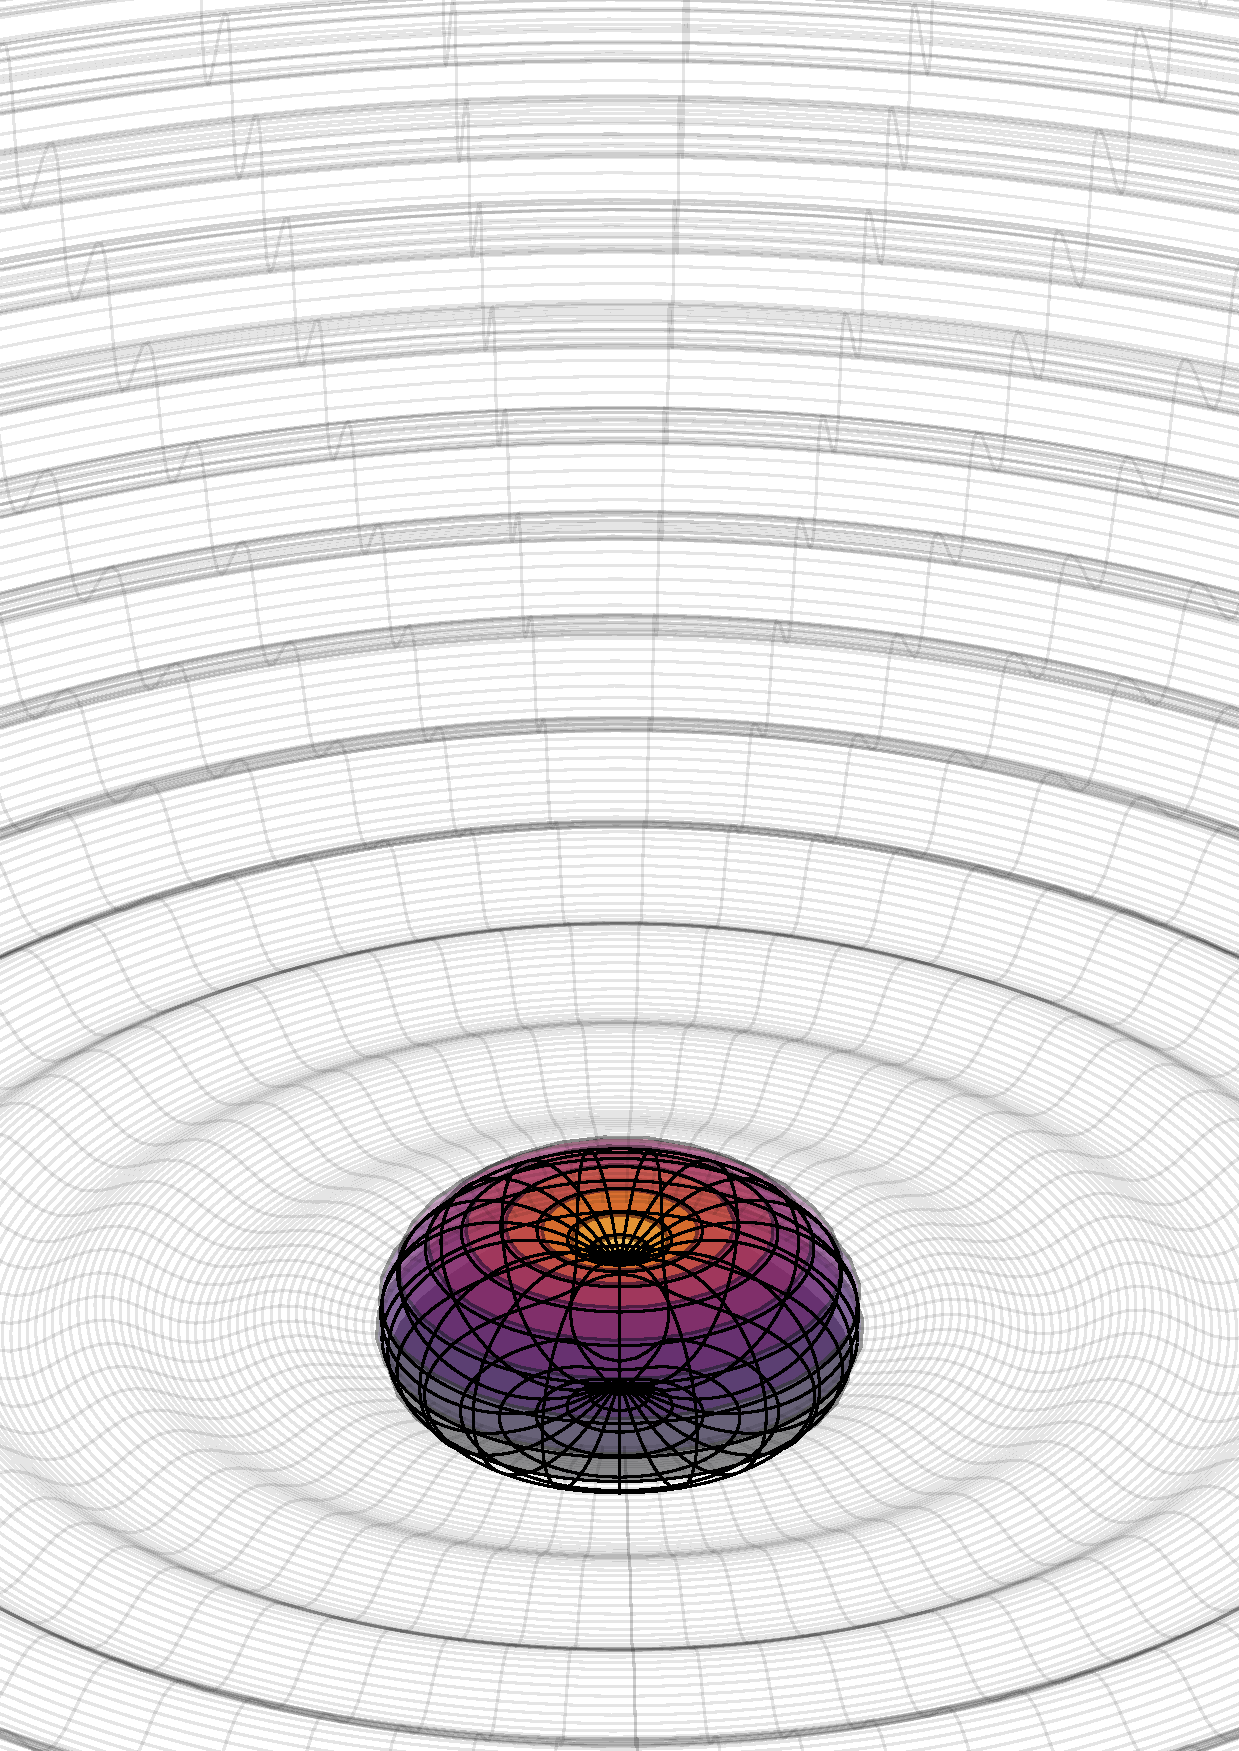
\includegraphics[width=\paperwidth, height=\paperheight]{figs/title2.pdf}};


        %{\fontsize{35}{55}\fontfamily{phv}\selectfont\bfseries X-ray bursts as a gauge for ultra-dense matter inside neutron stars}
    \begin{center}
        {\fontsize{30}{55}\fontfamily{phv}\selectfont\bfseries X-ray Bursts as a Tool to Constrain the Equation of State of the Ultra-Dense Matter Inside Neutron Stars}

    %\noindent\makebox[\linewidth]{\rule{\paperwidth}{2.4pt}}
    \phantom{Blaa!}

    \LARGE\fontfamily{phv}\selectfont\bfseries Joonas Nättilä
    \end{center}


\end{titlepage}

\restoregeometry
